
\section{Implementation}

In this section, we give a brief introduction of the big data technologies to be used in implementing 
our proposed system, namely, Apache Flink and Apache Kafka.  

We are planing to implement the proposed system over Apache Flink which provides the distributed stream processing components of the distributed predictors, alongside  Apache kafka for streaming the input event streams, and as a messaging platform to enable the distributed online learning functionalities. Figure \ref{fig:system_arch} illustrates the general architecture and implementation of the proposed large-scale patterns prediction system.

\begin{figure}[!ht]
	\begin{centering}
		
		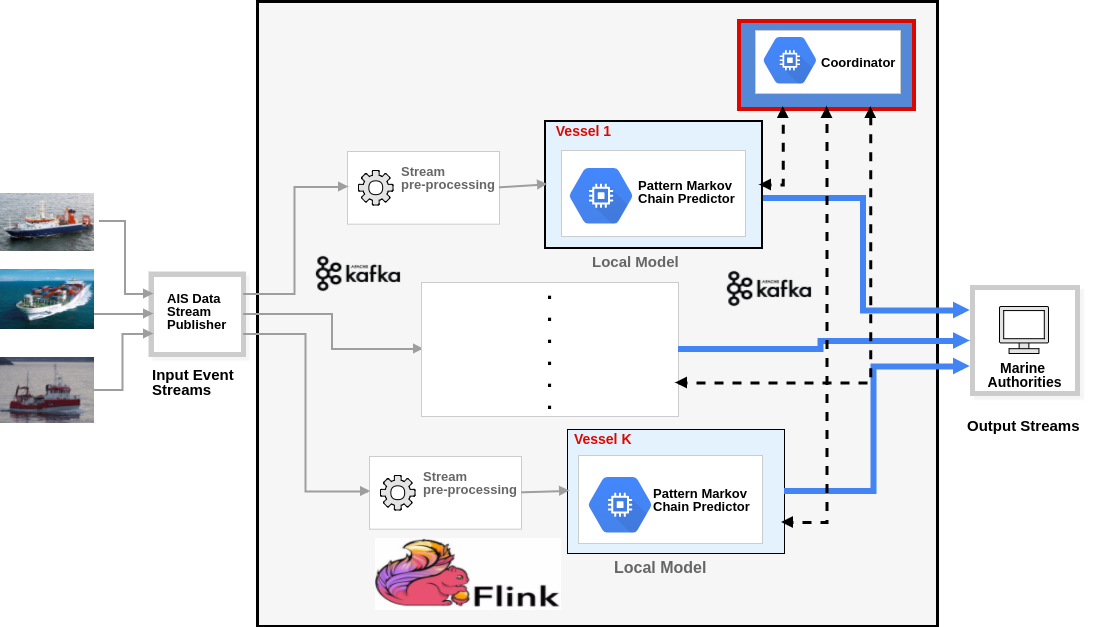
\includegraphics[width=0.9\textwidth]{figures/architecturedist.png}	
		
		%\hfill
		\caption{An Overview of Our Proposed System Architecture and  Implementation}  
		\label{fig:system_arch}
	\end{centering}
\end{figure} 

\subsection{Apache Flink}
 Apache Flink is an open source project that provides a large-scale, distributed and stateful stream processing platform \cite{carbone2015apache}. Flink is one of the recent and common big data processing frameworks, it employees data-stream processing model for streaming and batch data, the batch processing is treated as a special case of streaming applications (i.e., finite stream). The Flink's software stack includes the  $DataStream$ and $DataSet$ APIs for processing infinite and finite data, respectively. These two core APIs built on the top of the Flink's core distributed streaming dataflow engine. Additionally, Flink provides libraries such as Complex event processing for Flink (Flink-CEP), Machine Learning for Flink (FlinkML) and Flink Graph API (Gelly) \cite{carbone2015apache}.
 
 \par The main data abstractions of Flink are $DataStream$ and $DataSet$ that represent read-only collection of data elements. The list of elements is bounded (i.e., finite) in $DataSet$, while it is unbounded (i.e., infinite) in the case of $DataStream$. The Flink's core is a distributed streaming dataflow engine, with each
 Flink program is represented by a data-flow graph (i.e., directed acyclic graph - DAG) that executed by the Flink's engine \cite{carbone2015apache}. The data flow graphs are composed of stateful (state is maintained per partition), parallel operations and intermediate data stream partitions.
 
\subsection{Apache Kafka}

Apache Kafka is scalable, fault-tolerant and distributed streaming framework \footnote{\url{https://kafka.apache.org/}}. It allows to publish and subscribe to arbitrary data streams. Kafka manages the stream records in different categories (i.e., topics) that are partitioned and distributed over the Kafka servers. It provides the ability to publish a stream of records to one or more Kafka topic, to be consumed by applications that can subscribe to one or more topic to read data streams. The stream is distribute and balance between receivers within the same group for the sake of scalability.